\section{Polarization}
This section is based on Section 1.7 of University Physics Volume 3 \cite[30-33]{lingUniversityPhysicsVolume2016}.
Light is an electromagnetic (EM) wave with oscillating electric and magnetic fields perpendicular to its direction of propagation.
The specific orientation of these oscillations is referred to as polarization.Natural light sources, such as the Sun, emit unpolarized light in which the electric fields have random orientations, encompassing various polarization directions.


Polarizing filters are capable of selectively transmitting light waves with polarization aligned with the filter's orientation, while blocking waves that are not aligned.
This behavior follows Malus's law, which describes the relationship between the intensity of polarized light transmitted through a polarizer and the angle between the polarization direction of the incident light and the orientation of the polarizer:
\begin{equation}
    I = I_0 cos^2 \theta
\end{equation}

\subsection{Polarization Properties of Reflected Light}
Unpolarized light becomes polarized when it is reflected off a surface \cite[34]{lingUniversityPhysicsVolume2016}.
This is the reason why sunglasses are commonly polarized, as they are designed to block reflected light from surfaces such as roads or water.
Figure \ref{fig:polarized_reflection} illustrates this phenomenon where the component of light with vertical polarization (parallel to the plane of incidence) is less reflected compared to the component with horizontal polarization (perpendicular to the plane of incidence).

\begin{figure}[H]
    \centering
    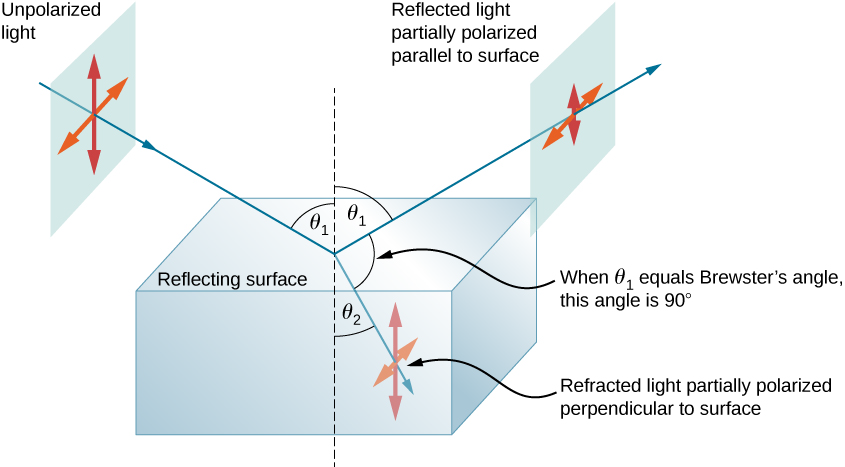
\includegraphics[width=\textwidth]{figures/polarization/reflaction.png}
    \caption{\blockquote{Polarization by reflection.
            Unpolarized light has equal amounts of vertical and horizontal polarization.
            After interaction with a surface, the vertical components are preferentially absorbed or refracted, leaving the reflected light more horizontally polarized.
            This is akin to arrows striking on their sides and bouncing off, whereas arrows striking on their tips go into the surface.}\cite[Figure 1.38]{lingUniversityPhysicsVolume2016}}
    \label{fig:polarized_reflection}
\end{figure}

The

\begin{align*}
    \centering
    r_\parallel = & \frac{\eta_1 \cos{\left(\theta_1 \right)} - \eta_2 \cos{\left(\theta_2 \right)}}
    {\eta_1 \cos{\left(\theta_1 \right)} + \eta_2 \cos{\left(\theta_2 \right)}}                        \\
    \\
    r_\perp     = & \frac{- \eta_1 \cos{\left(\theta_2 \right)} + \eta_2 \cos{\left(\theta_1 \right)}}
    {\eta_1 \cos{\left(\theta_2 \right)} + \eta_2 \cos{\left(\theta_1 \right)}}
\end{align*}

Where $r_\parallel$ and $r_\perp$ are the reflection coefficients for the lighe with a polarization parallel and perpendicular to the plane of incidence respectively.
$\eta_1$ is the refractive index of the air, $\eta_2$ is the refractive index of the water.
$\theta_i$ is the angle of incidence and $\theta_r$ is the angle of refraction.

Using the trigonometric identity $ \cos^2{\left(\theta_2 \right)} = 1- \sin^2{\left(\theta_2 \right)}$ and Snell's law $\eta_1 \sin{\left(\theta_1 \right)} = \eta_2 \sin{\left(\theta_2 \right)}$ the reflection coefficients angle of refrection can be removed and the equations can be written as:

\begin{align}
    r_\parallel = & \frac{\eta_1 \cos{\left(\theta_1 \right)} - \sqrt{- \eta_1^{2} \sin^{2}{\left(\theta_1 \right)} + \eta_2^{2}}}
    {\eta_1 \cos{\left(\theta_1 \right)} + \sqrt{- \eta_1^{2} \sin^{2}{\left(\theta_1 \right)} + \eta_2^{2}}}                                   \\
    \\
    r_\perp     = & \frac{- \eta_1 \sqrt{- \eta_1^{2} \sin^{2}{\left(\theta_1 \right)} + \eta_2^{2}} + \eta_2^{2} \cos{\left(\theta_1 \right)}}
    {\eta_1 \sqrt{- \eta_1^{2} \sin^{2}{\left(\theta_1 \right)} + \eta_2^{2}} + \eta_2^{2} \cos{\left(\theta_1 \right)}}
\end{align}

\begin{figure}[H]
    \centering
    \subcaptionbox{Mean value of polarization images.}{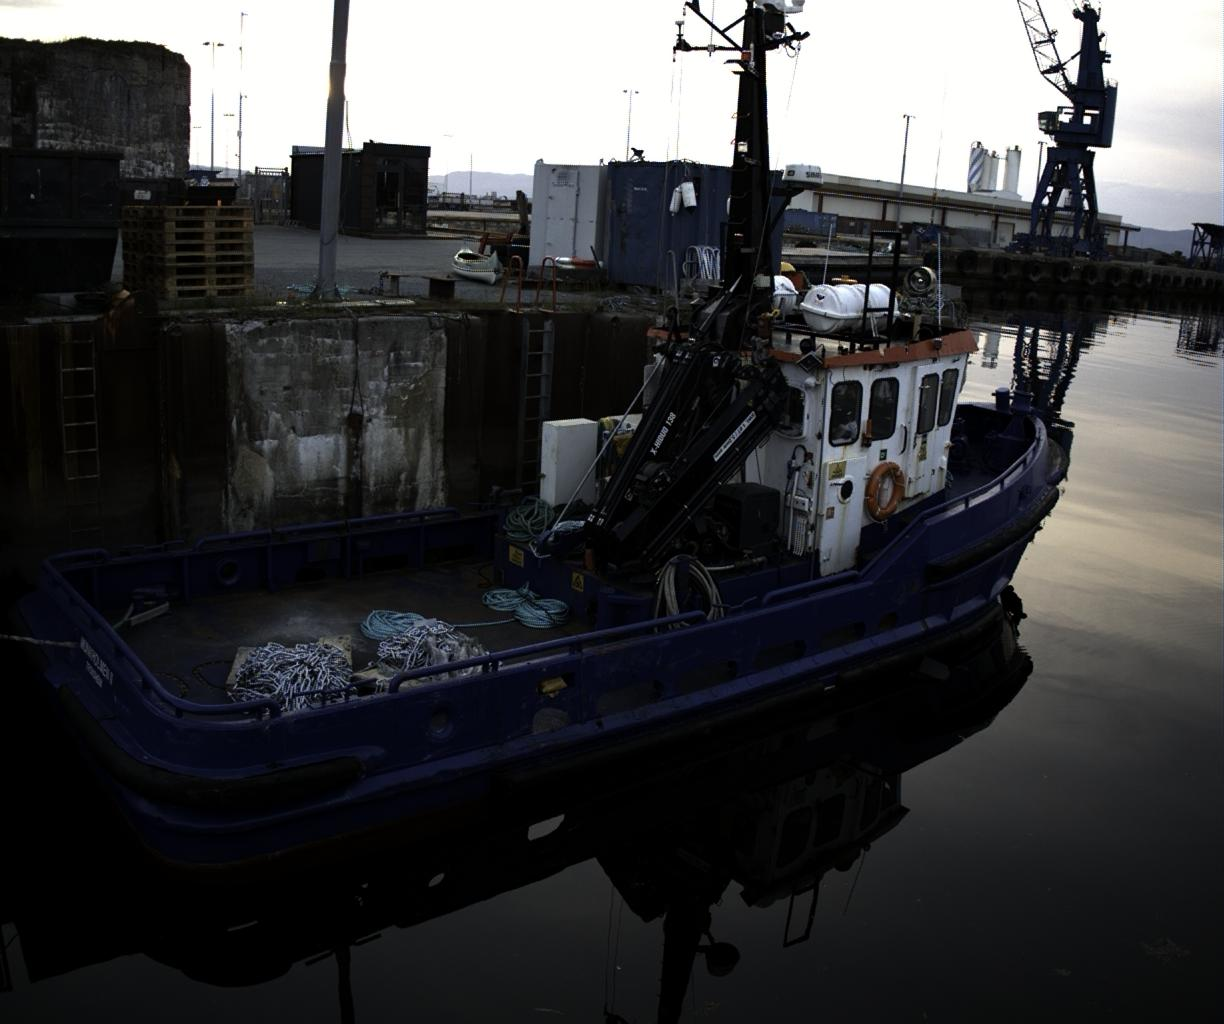
\includegraphics[width=.8\textwidth]{figures/pictures/regular_left_231.jpeg}}
    \subcaptionbox{HSV visualization of polarization data where the angle of polarization is encoded as hue and degree of polarization is encoded as value.}{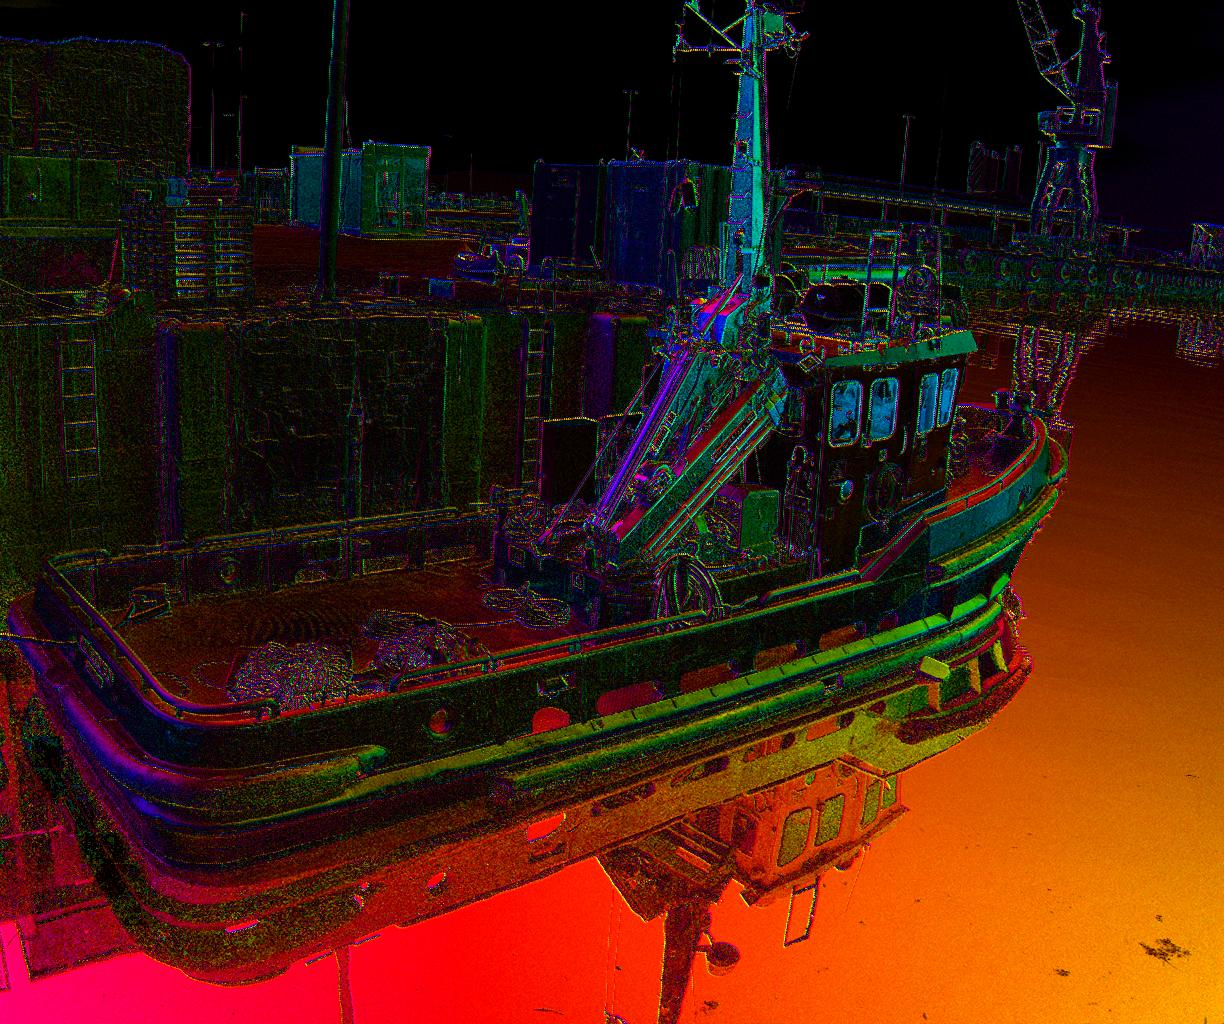
\includegraphics[width=.8\textwidth]{figures/pictures/aolp_left_231.jpeg}}
    \caption{Visualization of }
\end{figure}

